\documentclass[tikz, margin=3.14mm]{standalone}
\usepackage{pgfplots}
\pgfplotsset{compat=1.18}
\usetikzlibrary{calc}

\begin{document}
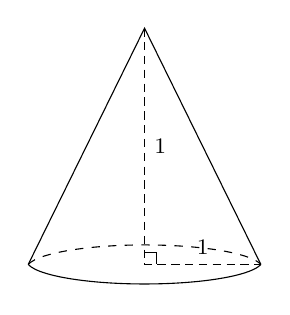
\begin{tikzpicture}[scale=.75]
    \draw[dashed] (0,0) arc (170:10:2cm and 0.4cm)coordinate[pos=0] (a);
    \draw (0,0) arc (-170:-10:2cm and 0.4cm) coordinate (b);
    \draw[densely dashed] 
        ([yshift=4cm]$(a)!0.5!(b)$) -- 
        node[right,font=\footnotesize] {1} coordinate[pos=0.95] (aa)($(a)!0.5!(b)$) -- 
        node[above,font=\footnotesize] {1} coordinate[pos=0.1] (bb) (b);
    \draw (aa) -| (bb);
    \draw (a) -- ([yshift=4cm]$(a)!0.5!(b)$) -- (b);
\end{tikzpicture}
\end{document}